\documentclass[letterpaper,12pt]{article}
\usepackage{tabularx} % extra features for tabular environment
\usepackage{amsmath}  % improve math presentation
\usepackage{float}
\usepackage{pdfpages}

\usepackage{graphicx} % takes care of graphic including machinery
\graphicspath{ {./figures/} }
\usepackage[margin=1in,letterpaper]{geometry} % decreases margins
\usepackage{cite} % takes care of citations
\usepackage[final]{hyperref} % adds hyper links inside the generated pdf file
\hypersetup{
	colorlinks=true,       % false: boxed links; true: colored links
	linkcolor=blue,        % color of internal links
	citecolor=blue,        % color of links to bibliography
	filecolor=magenta,     % color of file links
	urlcolor =blue         
}

%



\begin{document}

\title{Experiment 4 \protect\\Resistive Circuits}
\author{Ahmet Akman 2442366 \protect\\ Assistant : Şirin Yazar}
\date{\today}
\maketitle

%\begin{abstract}
%abstract
%\end{abstract}

\section{Introduction} 
In this experiment, as students, we are expected to experiment with how to use measure voltage, current, and resistance by completing the steps described in the third experiment laboratory manual. Throughout these steps, how to determine the resistance via reading resistor color codes and using a multimeter is expected to be learned. As students, we are expected to discriminate the analog and digital multimeters by considering their internal voltage sources. It is observed how to measure the AC line voltage. How to measure DC current and voltage, how the potentiometer works, the characteristics of linear and non-linear resistors, and equivalent resistances are observed by connecting the multimeters directly to each other and the circuit. The results of the steps were noted and plotted for further comments.
\section{Experimental Results}
In this section, the results of Experiment 4 are discussed.
\subsection{Step 1}
\subsubsection{a} In this step, power supply, signal generator and oscilloscope instruments are used. The circuit given in Figure 1 is constructed. The \(V_{pp}\) is selected as 12 and the frequency is adjusted as 50 Hz. The channel 2 of the oscilloscope is connected to the terminals of rightmost resistor. 
\begin{figure}[H]
	\centering
   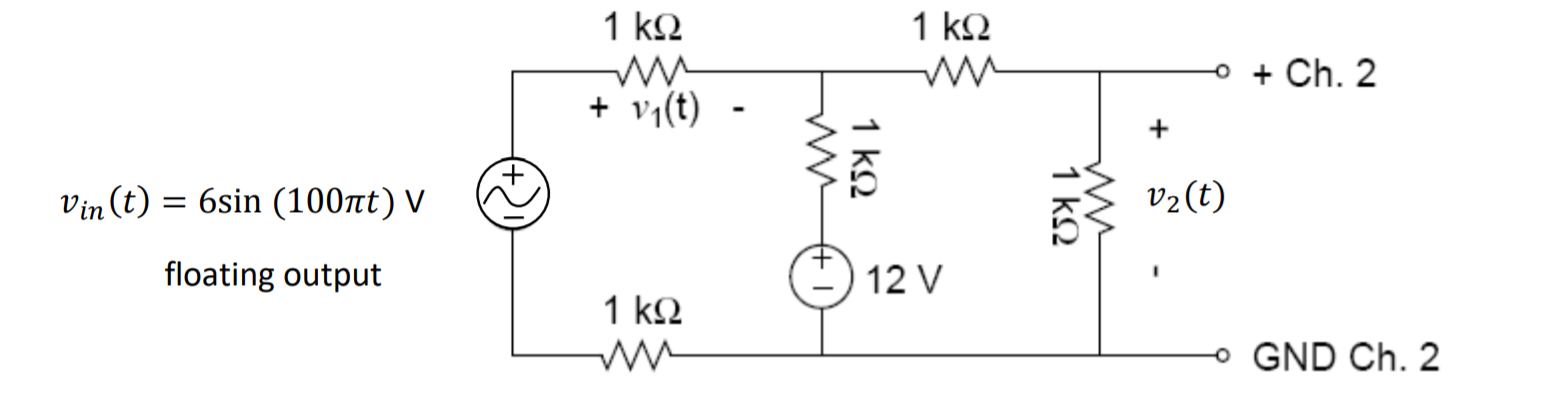
\includegraphics[width=0.6\textwidth]{1a_sch.png}
   \caption{Circuit schematic for the step 1 section \(a\)}
\end{figure} 
As a result the \(V_2(t)\) is observed and plottted. The plotting is given in the Figure 2. 
\begin{figure}[H]
	\centering
   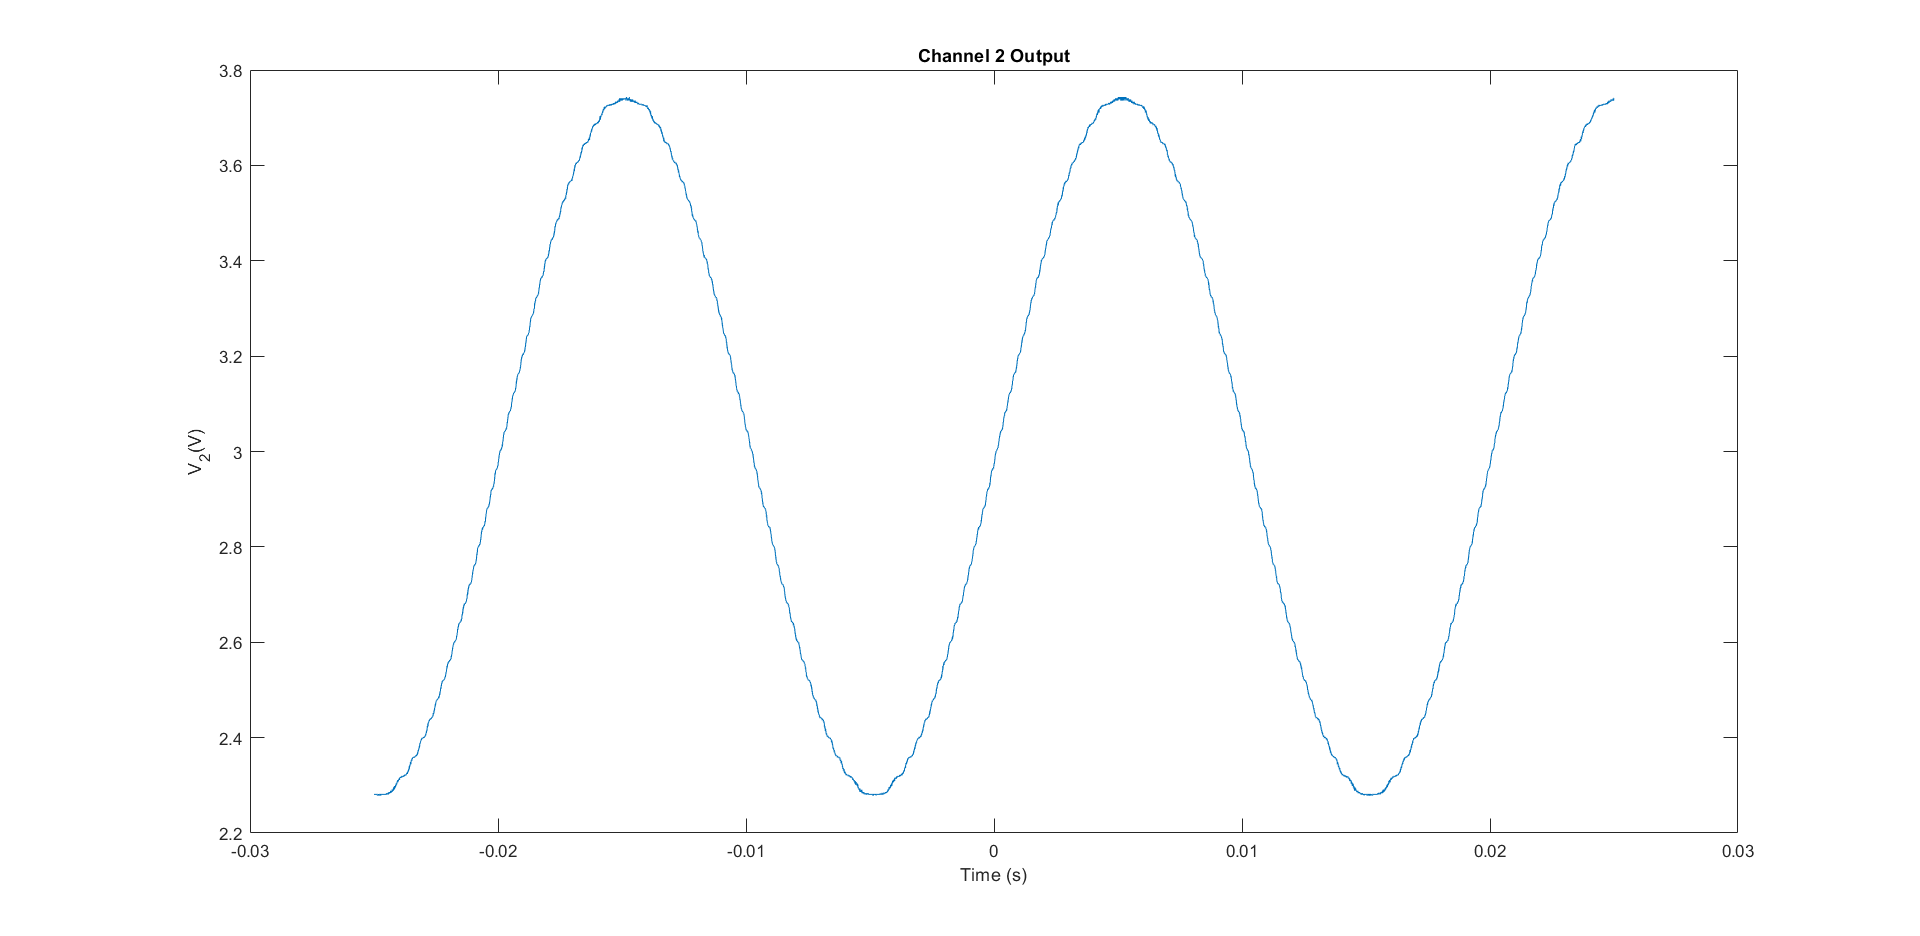
\includegraphics[width=1\textwidth]{1a.png}
   \caption{\(V_2\) versus time\((s)\) }
\end{figure} 


\subsubsection{b} 
In this step, the circuit given in in Figure 1 is used. As measurement setup, probes of the channel 1 is connected additionally. The setup is given in Figure 3. 

\begin{figure}[H]
	\centering
   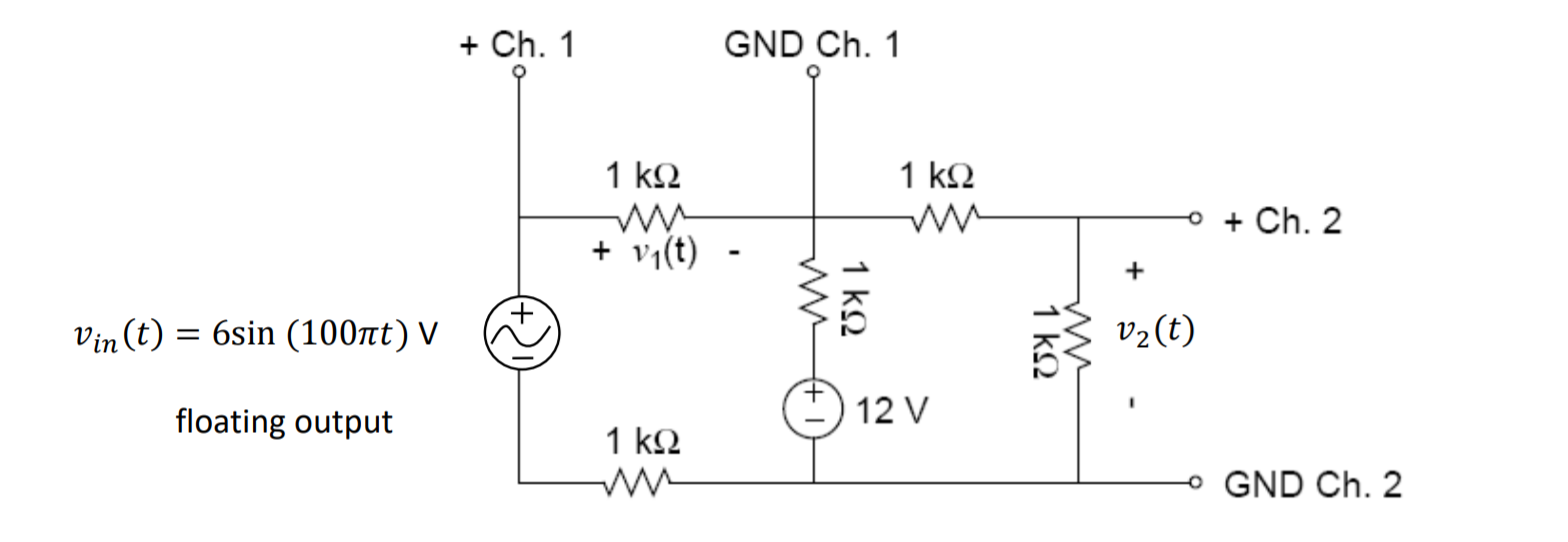
\includegraphics[width=0.6\textwidth]{1b_sch.png}
   \caption{Circuit schematic for the step 1 section \(b\)}
\end{figure} 

As a result the values of \(V_1\) and \(V_2\) are observed and plotted. The plotting is given in Figure 4. 
\begin{figure}[H]
	\centering
   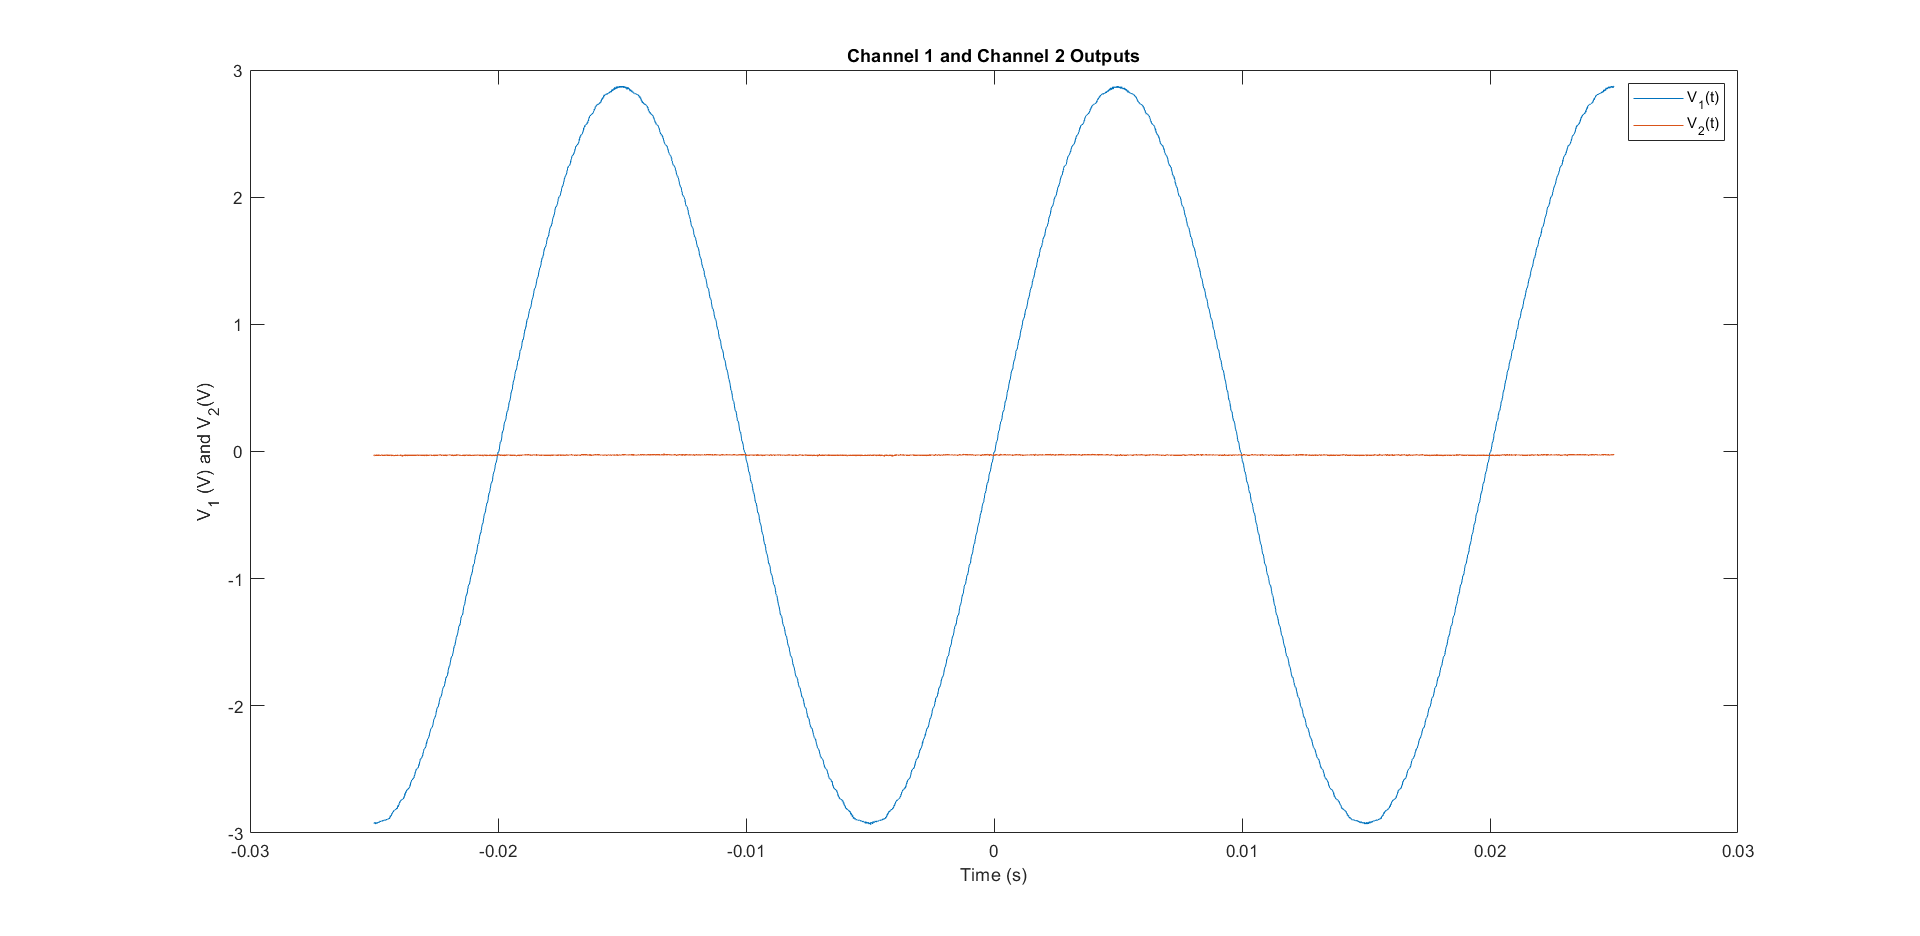
\includegraphics[width=1\textwidth]{1b.png}
   \caption{\(V_1\) \(V_2\) versus time\((s)\) }
\end{figure} 

As it can be seen from the plot channel 2 is approximately corresponds to "0" value , although it is not supposed to be so. The measurement probe of the second channel is connected between two ground terminals of the oscilloscope. This result demonstares that grounding configuration of the oscilloscope may prevent the accurate observations. 

For comparison the values measured and calculated therotically are given in the Table 1.
\begin{table}[H]
	\begin{center}
		\caption{Calculated values and measured values.}
		\vspace{2mm}
		\begin{tabular}{||c | c | c||} 
		 \hline 
		 X & Calculated (V) & Measured (V) \\ [0.5ex] 
		 \hline\hline
		 \(V_1\) & \( \frac{9}{5} \sin {100 \pi t } -3 \) & 1.5275  \\ 
		 \hline
		 \(V_2\) & \( \frac{3}{4} \sin {100 \pi t } +3 \) & 7.477  \\
		 \hline
		\end{tabular}
	\end{center}
\end{table}

\subsection{Step 2}
In Step 2, the circuit diagram given in the Figure 5 is constructed in the LTspice environment. Measurement probe nodes are indicated with texts on the figure.
\begin{figure}[H] \centering{
	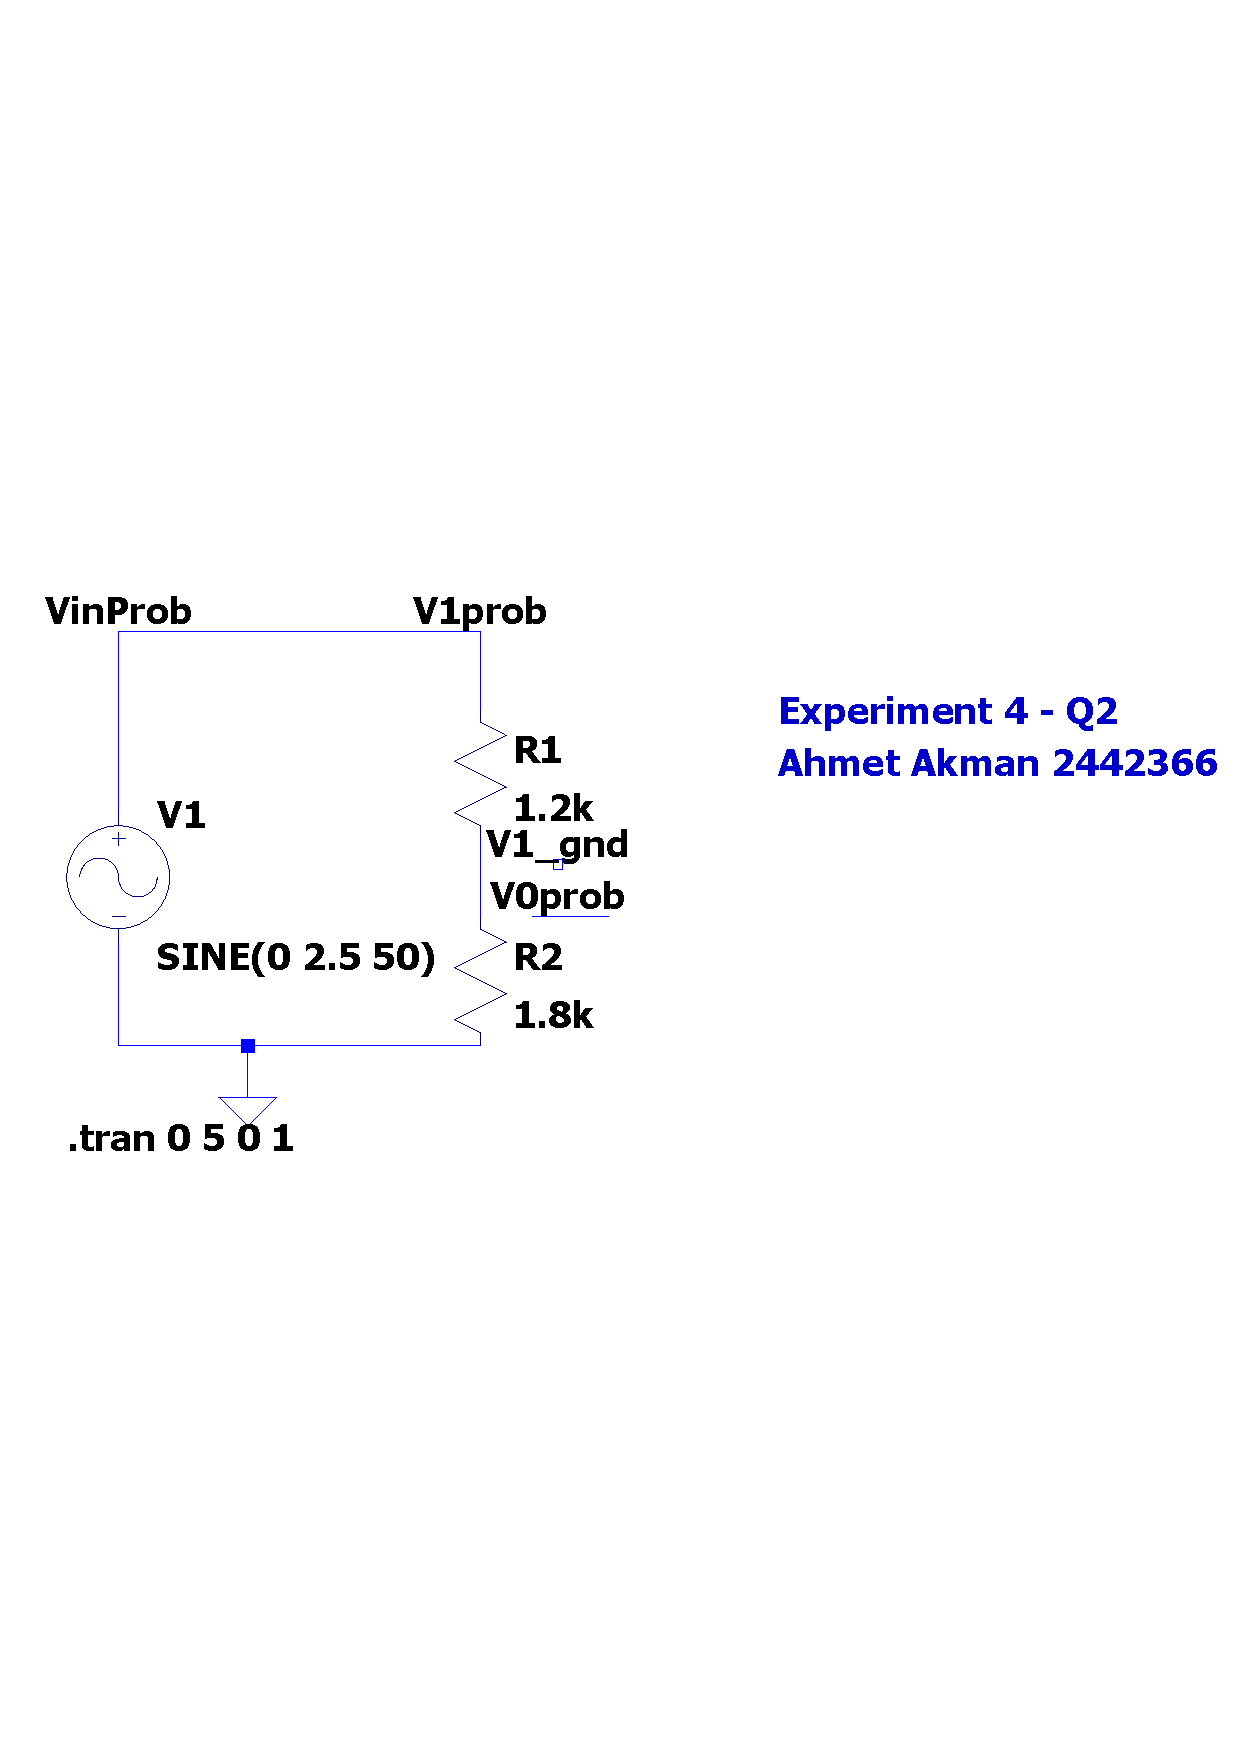
\includegraphics[scale=0.45]{2a_sch.pdf}}
	\caption{The circuit diagram for the Step 2}
\end{figure}

\subsubsection{a}
For the drawn circuit, \(V_{in}\) is set as 50 Hz and 5 \(V{pp}\). As a result the plot given in Figure 6 is obtained.
\begin{figure}[H] \centering{
	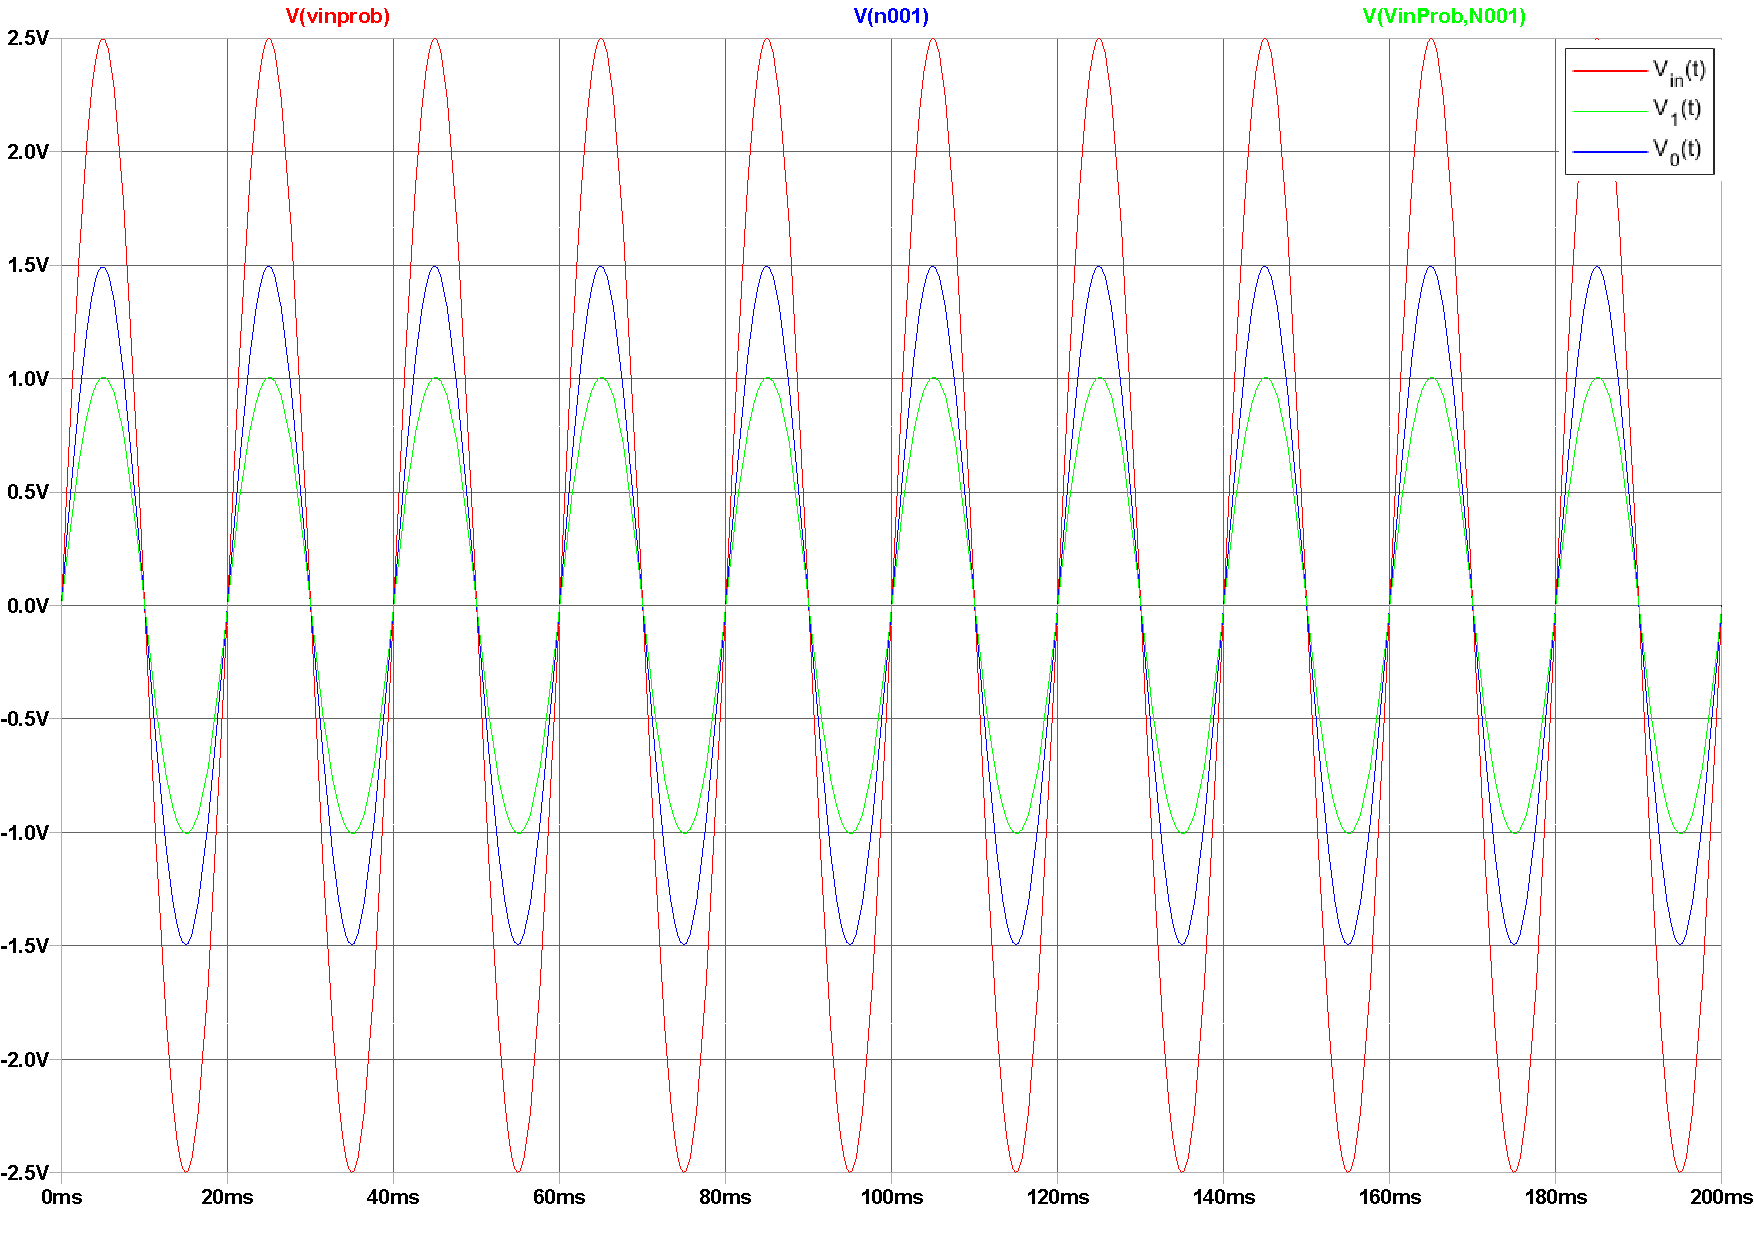
\includegraphics[scale=0.45]{2a_plot.pdf}}
	\caption{The plot of \(V{in}\) \(V_0\) \(V_1\) versus time(ms) }
\end{figure},

\subsubsection{b}
When the \(V_{in}\)  is displayed only it can be said that \(V{pp}\) is equal to "2" volts which is the same amplitude we found in part a. 


\subsection{Step 3}
In this step, signal generator and oscilloscope instruments are used. The circuit given in the Figure 7 is constructed.
\begin{figure}[H]
	\centering
   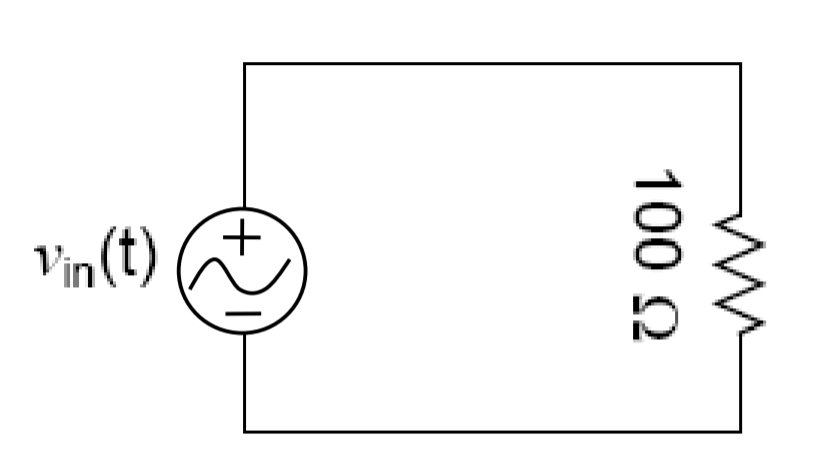
\includegraphics[width=0.5\textwidth]{3_sch.png}
   \caption{\(V_{in}\) versus time \((s)\) }
\end{figure}  

Before connecting the signal generator to the circuit , the terminals are directly connected to the oscilloscope probes. Then the observations are made ,and the output is given in the Figure 8. The \(V{pp}\) is measured as 3 volts.

\begin{figure}[H]
	\centering
   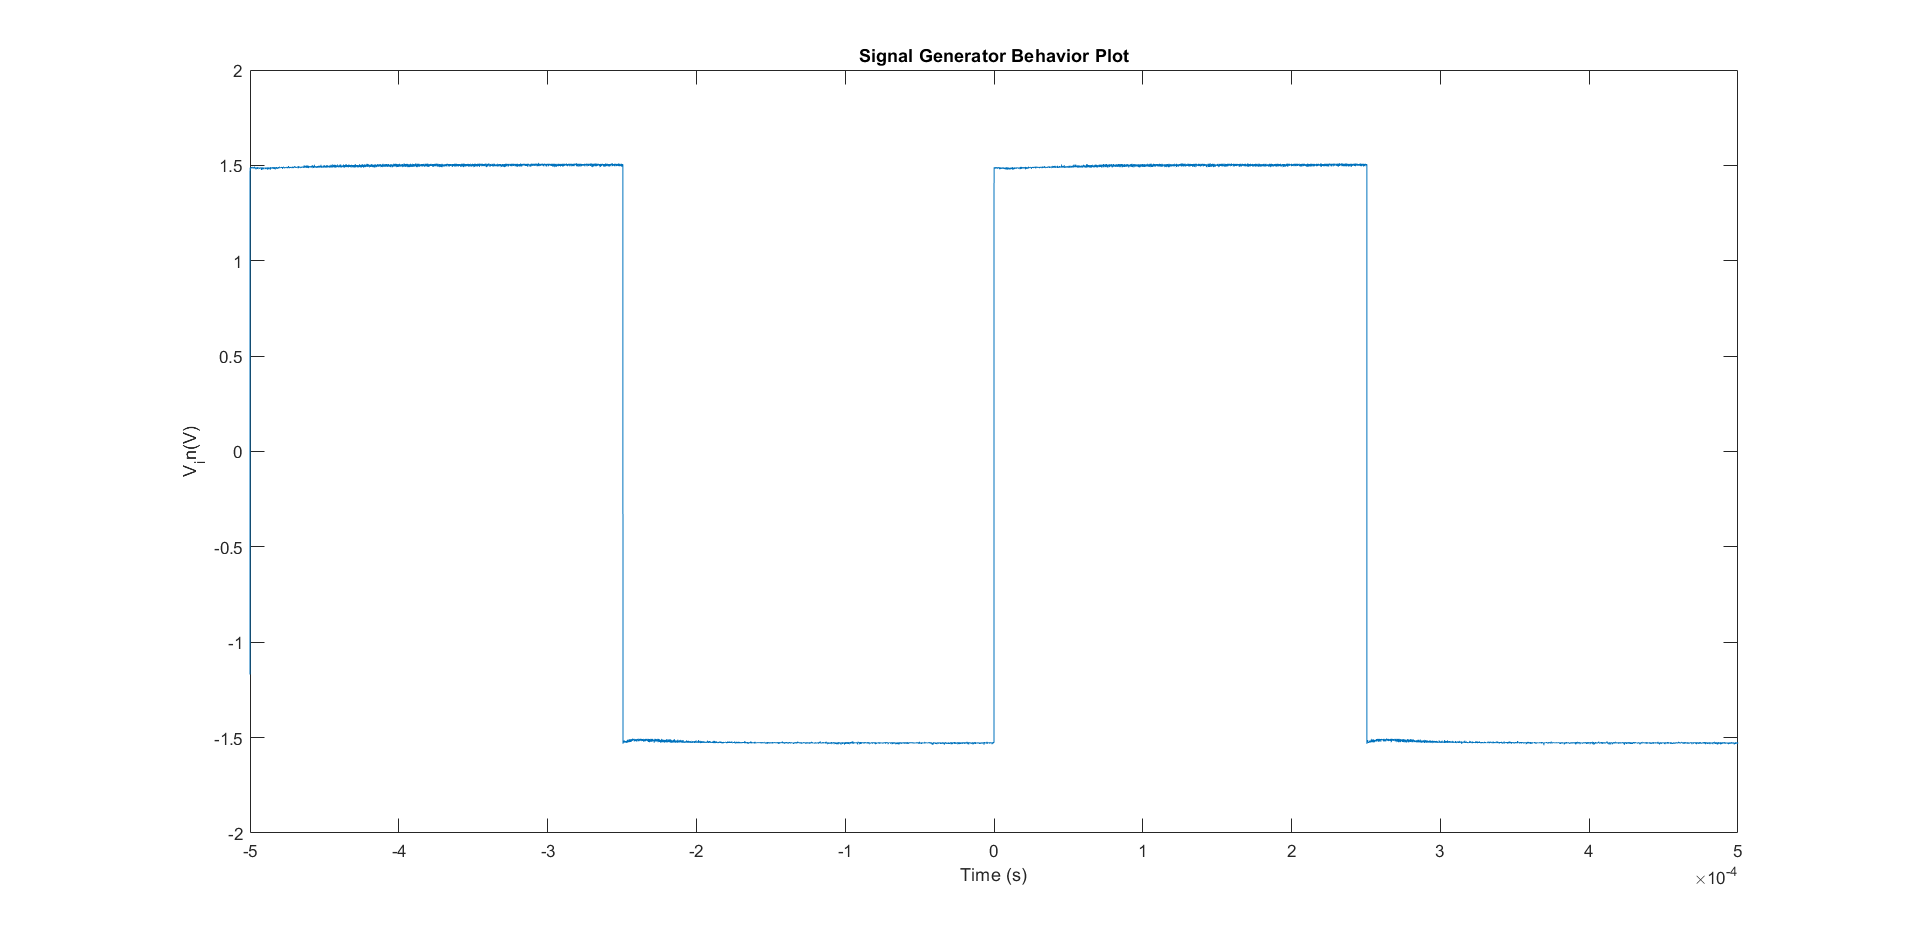
\includegraphics[width=1\textwidth]{3a.png}
   \caption{\(V_{in}\) versus time \((s)\) }
\end{figure}  

The signal generator is connected to the circuit. The measurements are displayed on the screen of DSO. Then the data  plotted are given in the Figure 9.
\begin{figure}[H]
	\centering
   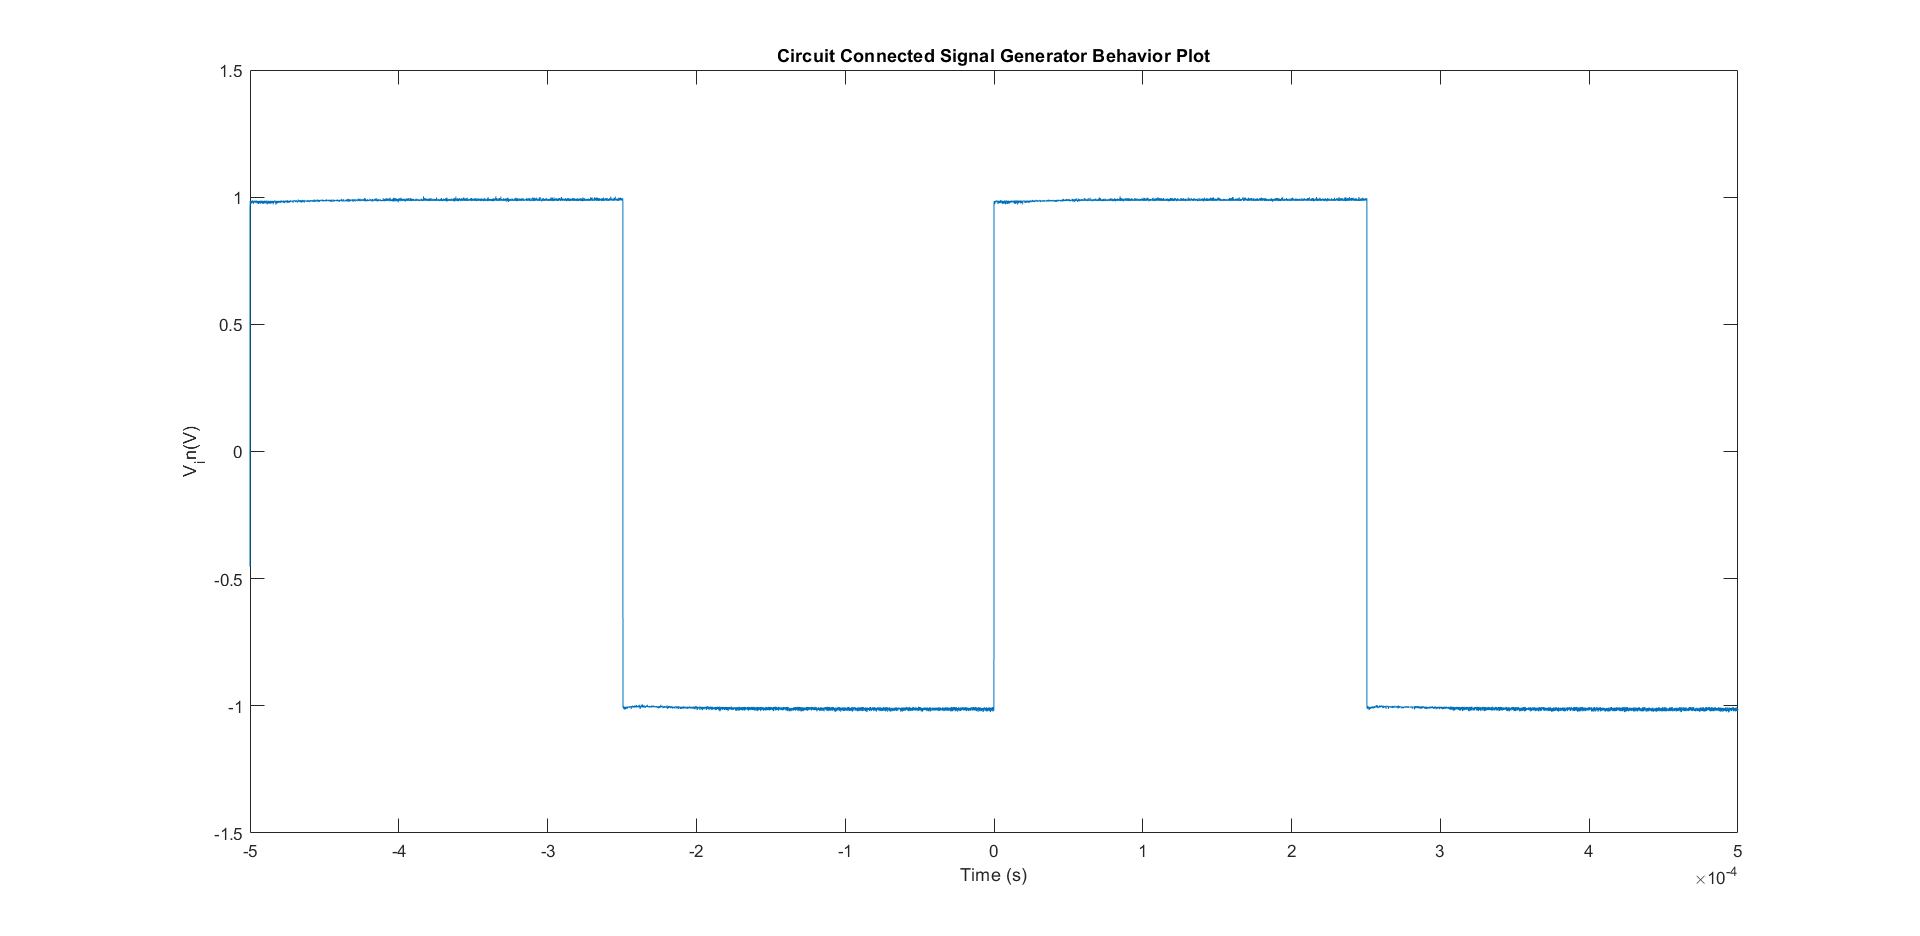
\includegraphics[width=1\textwidth]{3b.png}
   \caption{\(V_{in}\) versus time \((s)\) }
\end{figure}  
As a result , it can  be seen that the drops in the amplitude is stemmed from the non-ideal behavior of the signal generator. It is said that the signal generator has a 50 \(\Omega\)  internal resistance, so when a comparable resisance is connected the voltage is divided. It can be seen from the Figure 9, amplitude is dropped to 3 volts.


\subsection{Step 4}
In this step, the circuits given in the Figure 10 are set. And the source voltage is measured as 5 volts. 
\begin{figure}[H]
	\centering
   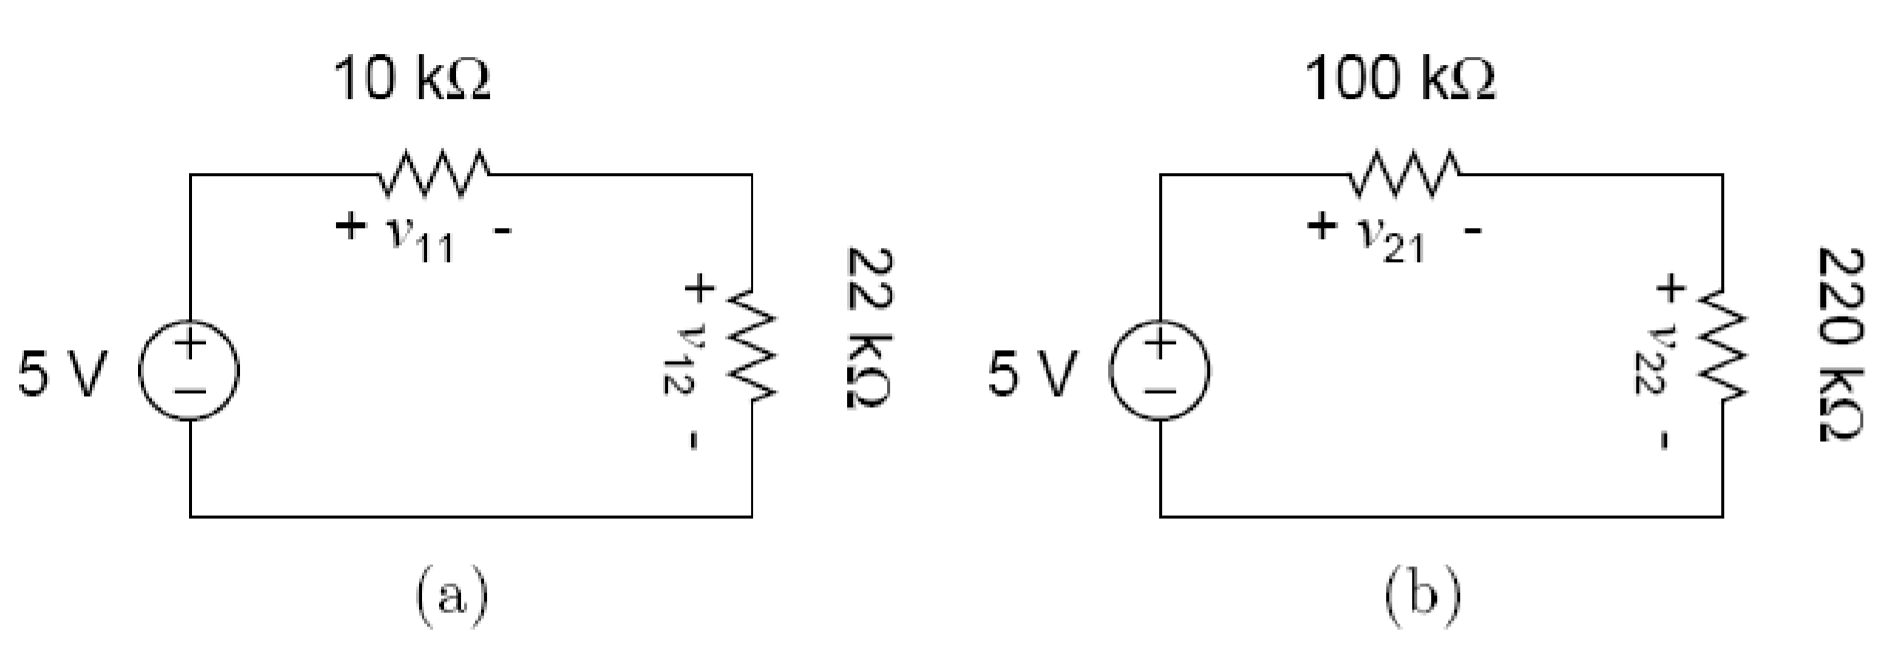
\includegraphics[width=1\textwidth]{4_sch.png}
   \caption{The circuit diagrams for the Step 4}
\end{figure}  

\subsubsection{a}
The  range of the analog multimeter is set to 5 V DC. The internal resistance of the analog multimeter is measured via digital multimeters resistance mode. The obtained internal resistance is "99.705k\(\Omega\)". All the voltage measurements are made using analog multimeter.
\subsubsection{b}
All the measurements are repeated and recorded using digital multimeter. For the comparison, the readings of the analog and digital multimeters are given in the Table 2.
\begin{table}[H]
	\begin{center}
		\caption{Analog and digital measurements}
		\vspace{2mm}
		\begin{tabular}{||c | c | c||} 
		 \hline 
		 X & Analog Reading (V) & Digital Reading (V) \\ [0.5ex] 
		 \hline\hline
		 \(V_{11}\) & 1.4 & 1.594  \\ 
		 \hline
		 \(V_{12}\) & 3.1 & 3.406  \\
		 \hline
		 \(V_{21}\) & 0.87 & 1.539  \\ 
		 \hline
		 \(V_{22}\) & 1.95 & 3.430  \\
		 \hline
		\end{tabular}
	\end{center}
\end{table}
There are two results can be inferred. Firstly, the analog multimeters measurements are quite inconsistent especially for the second circuit. This can be stemmed from the fact that the internal resistance of the analog multimeter is measured as a comparable value to the equivalent resistance of the second circuit. Secondly, the digital multimeter measures more accurate than the analog multimeter. The reason is that the digital multimeter can adjust its internal resistance so that the measurements are made properly.  

\subsection{Step 5}
\subsubsection{a}
In Step 2, the circuit diagram given in the Figure 11 is constructed in the LTspice environment.
\begin{figure}[H] \centering{
	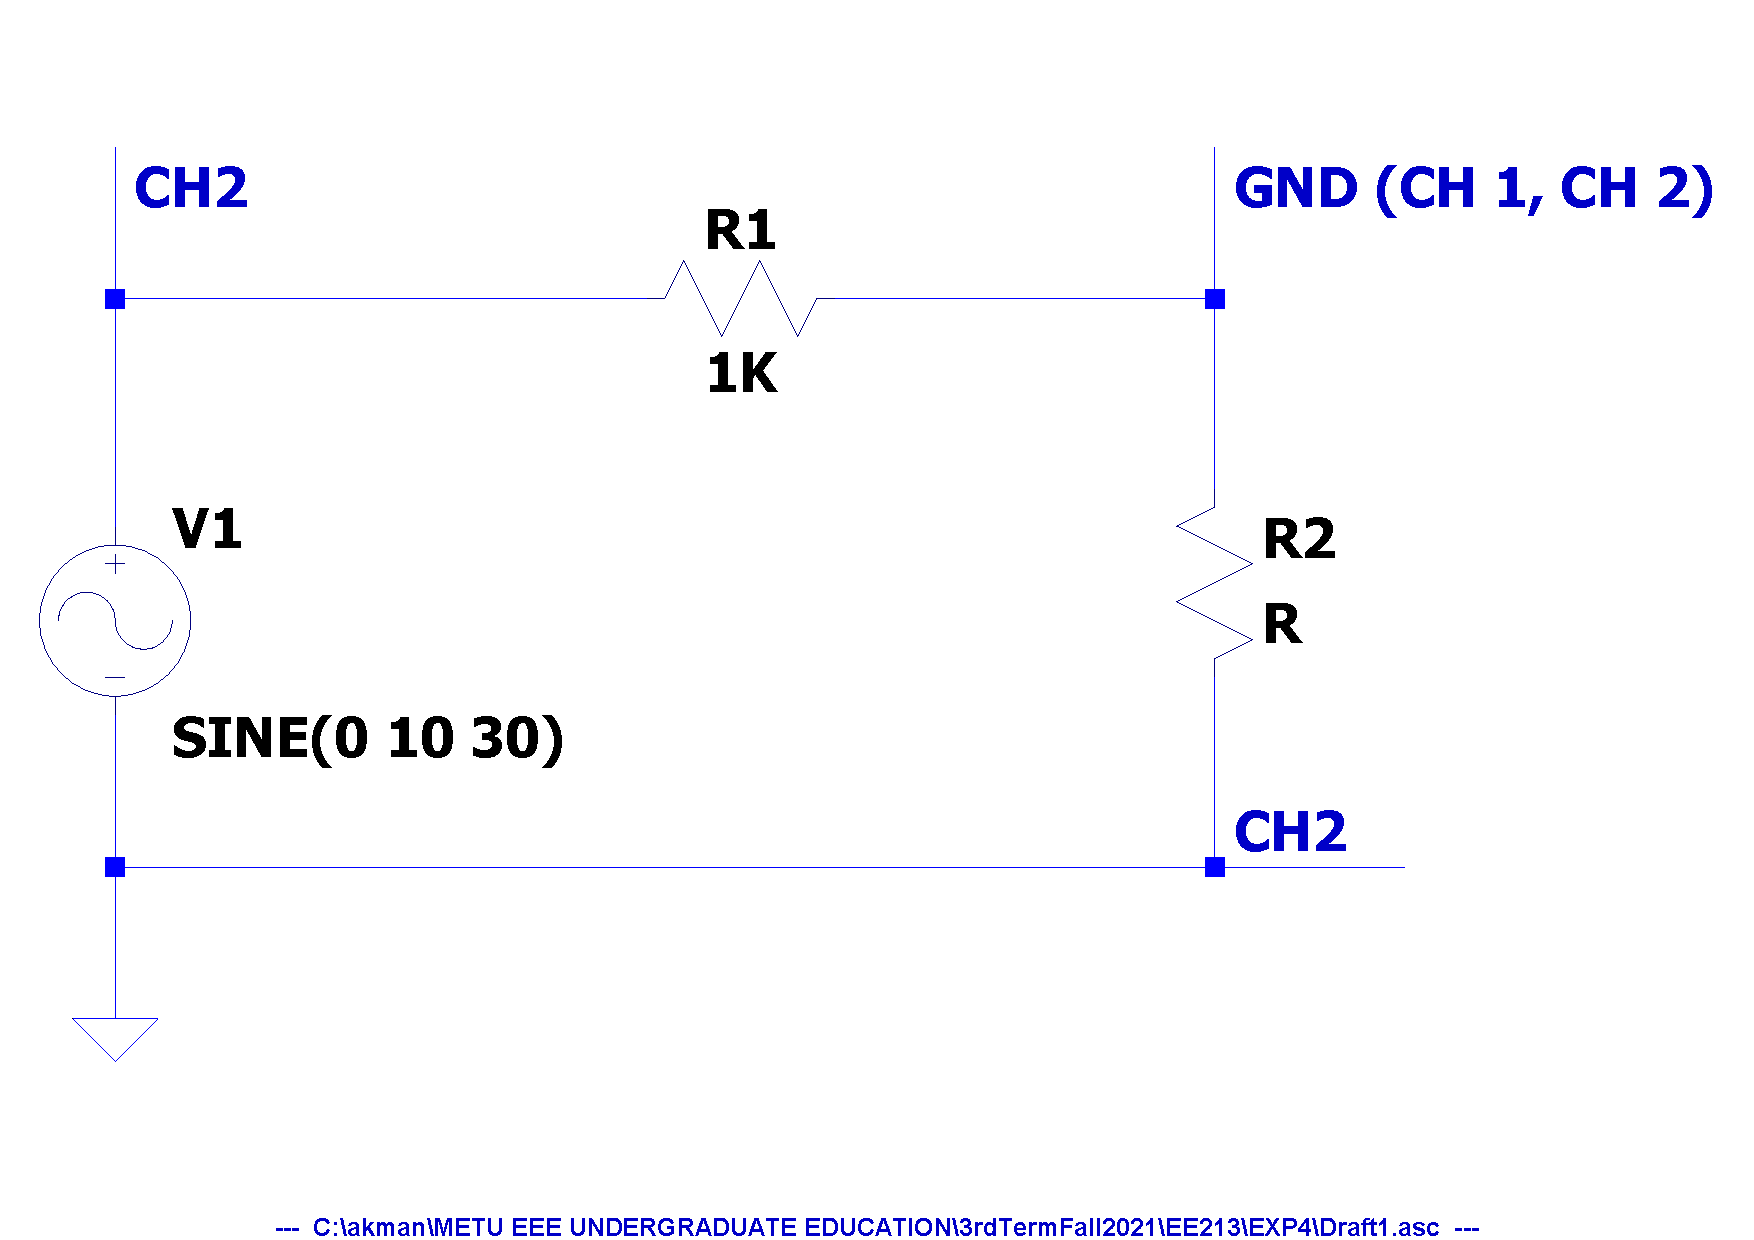
\includegraphics[scale=0.25]{5a.pdf}}
	\caption{The LTspice diagram for Step 5 part a }
\end{figure}
The resistance values are selected as 1K , 5K and 10K. Then the simulation is run, the data is fetched from the LTspice and plotted at the MATLAB. The plot can be seen from the Figure 12.

\begin{figure}[H]
	\centering
   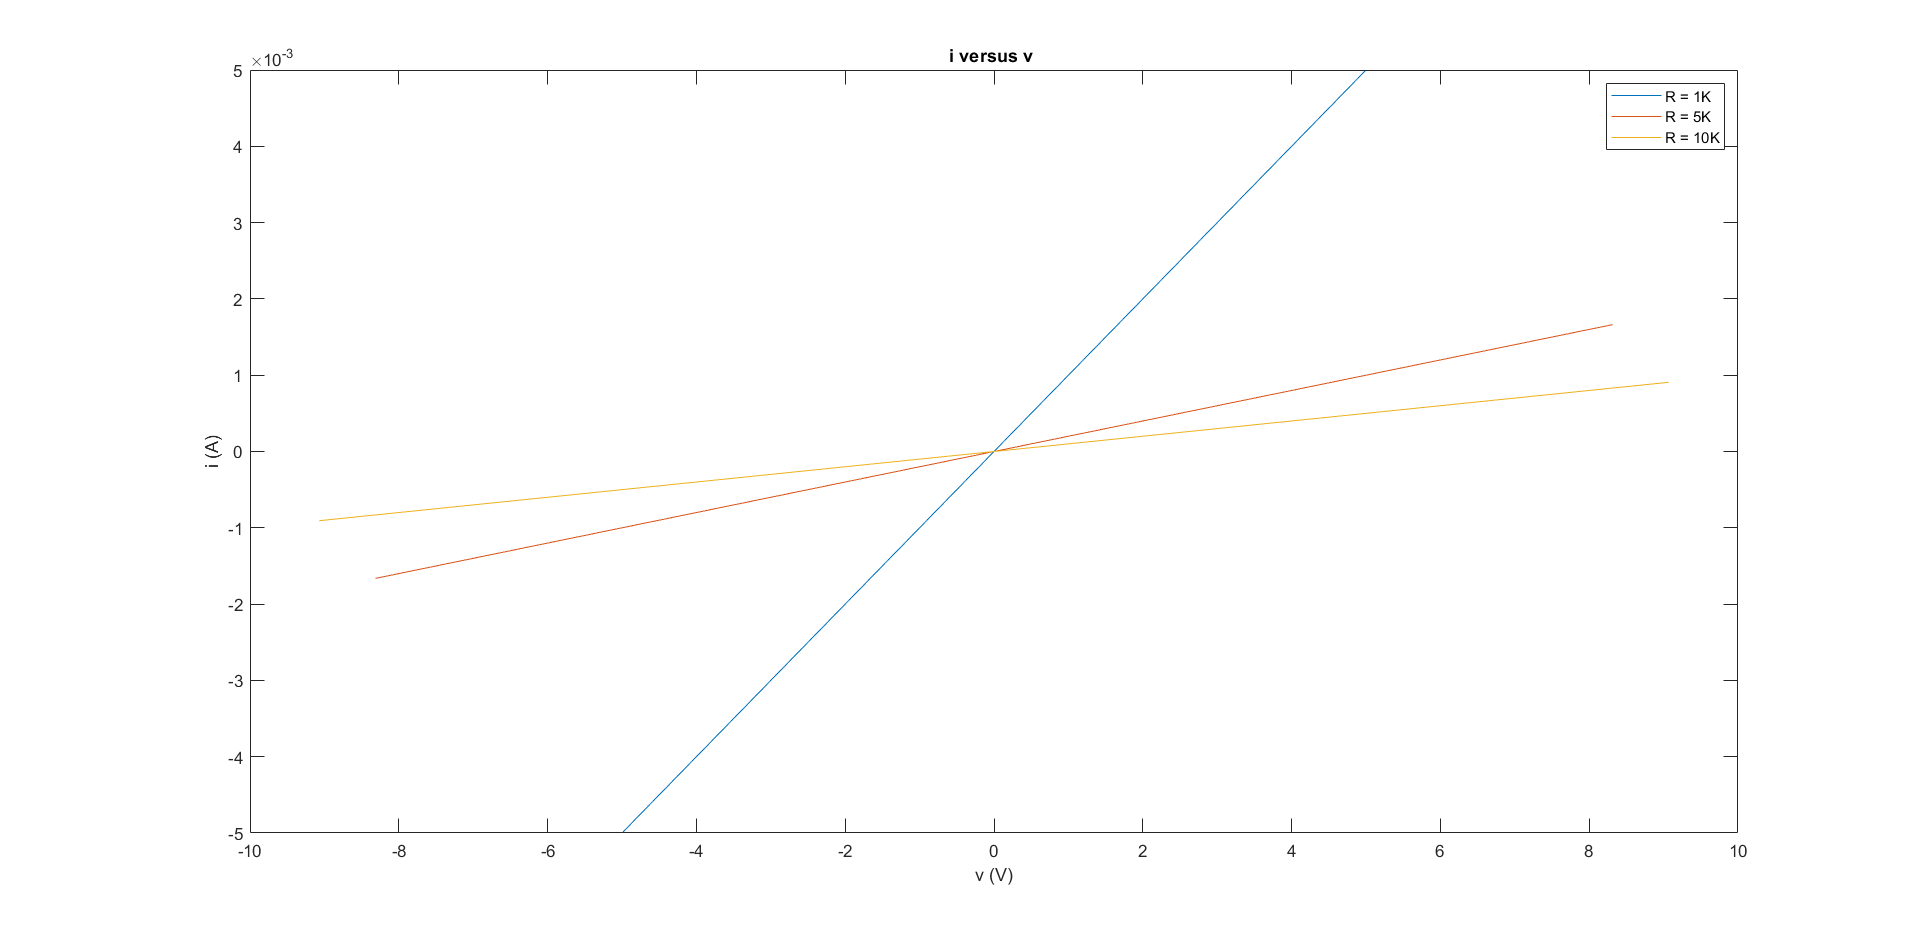
\includegraphics[width=1\textwidth]{5a.png}
   \caption{i versus v plot}
\end{figure}  
We can obtain the resistance values from the slope of the i-v lines. We can get the  current throught unknown R via directly CH2 measurement. We had to invert the CH1 to get i versus v characteristic in XY mode.

\subsubsection{b}
In the part b, the circuit diagram given in the Figure 13 is constructed in the LTspice environment.

\begin{figure}[H] \centering{
	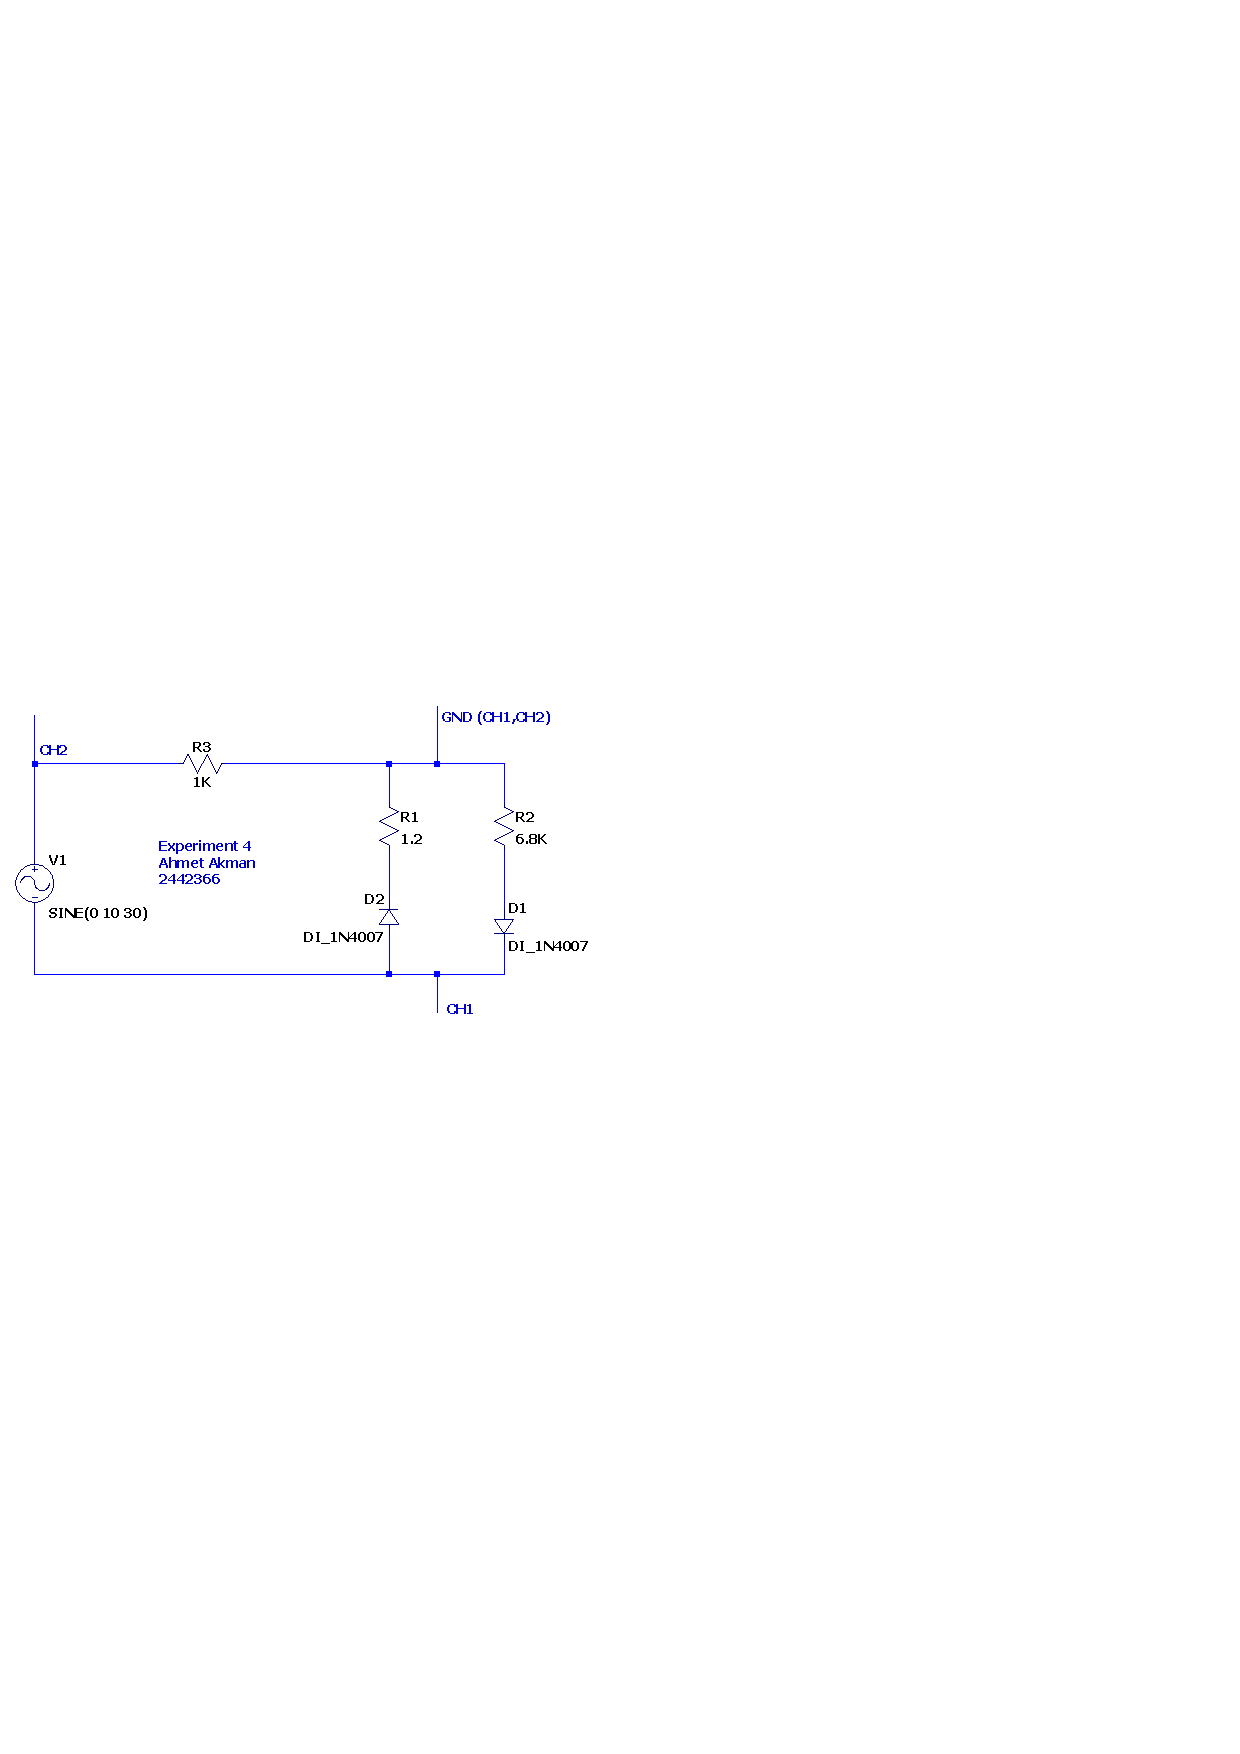
\includegraphics[scale=0.65]{5b.pdf}}
	\caption{The LTspice diagram for Step 5 part b}
\end{figure}
The simulation is rerun, the data is fetched from the LTspice and plotted at the MATLAB. The plot can be seen from the Figure 14.

\begin{figure}[H]
	\centering
   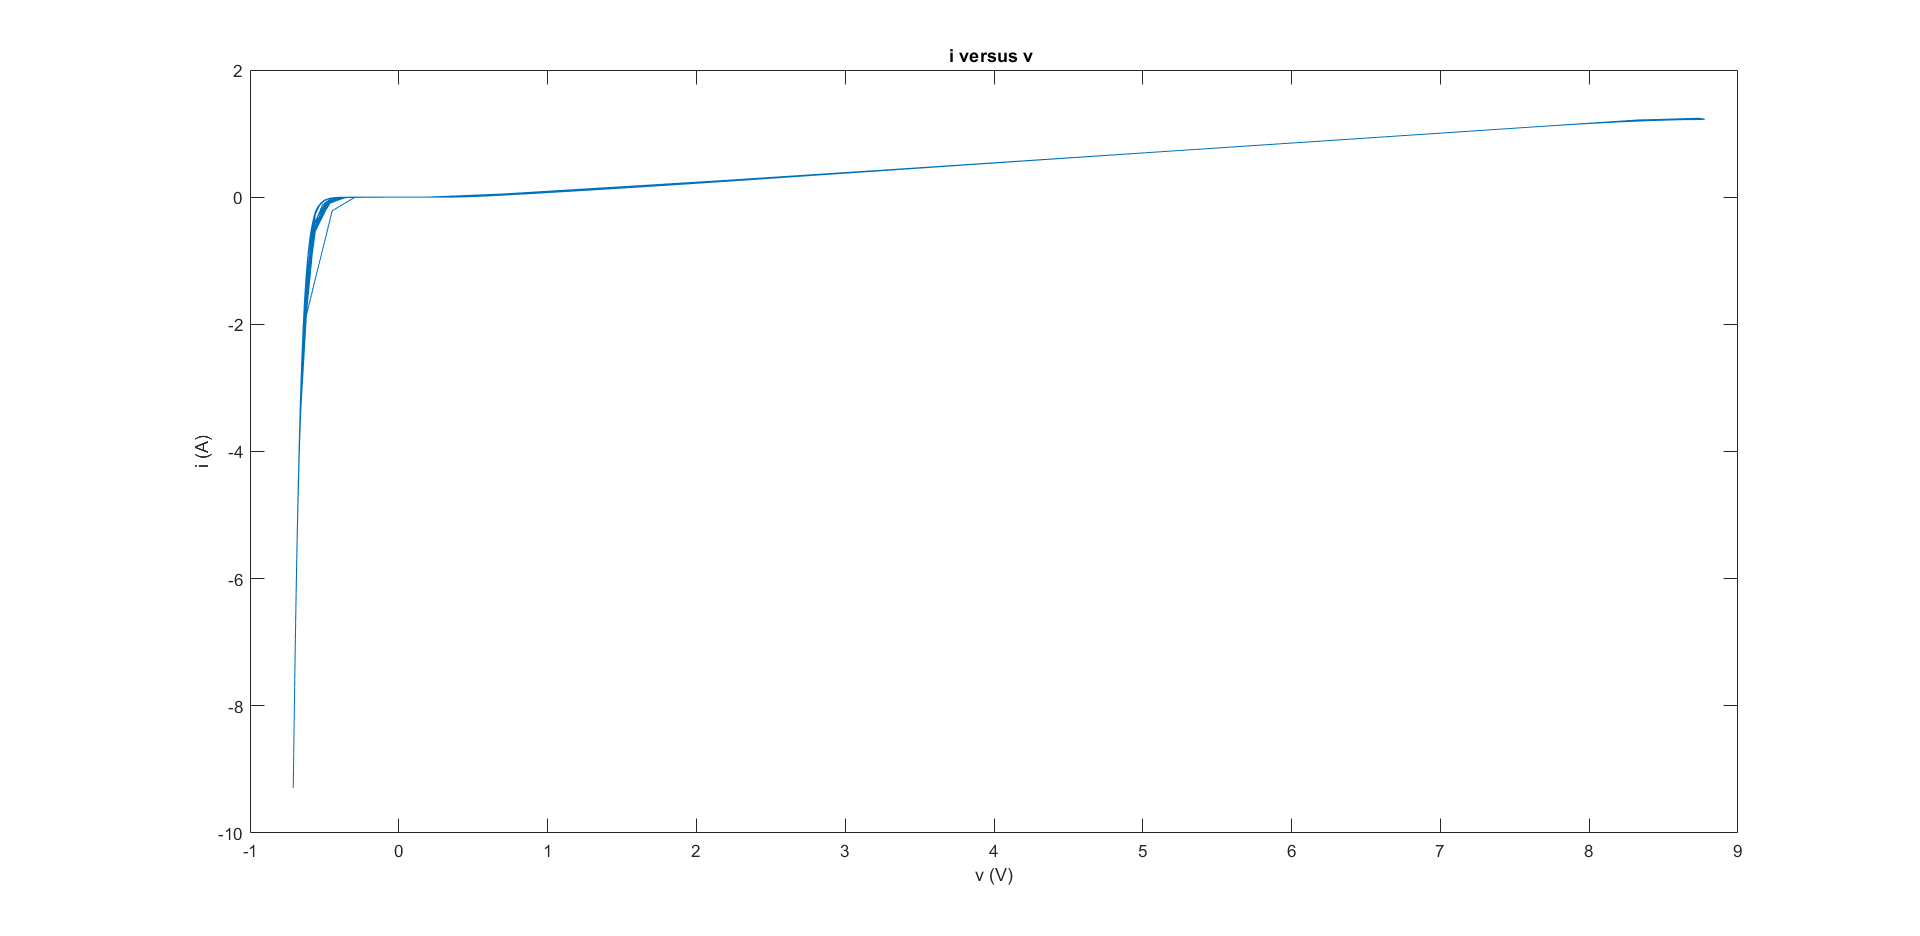
\includegraphics[width=1\textwidth]{5b.png}
   \caption{i versus v plot}
\end{figure}  
We can conclude from the plot that the equivalent resistance changes when the voltage direction change. The non ideal behavior is stemmed from 0.7 V tolerance of the diodes.


\subsection{Step 6}
In this step the Wheatstone Bridge circuit in the Figure 15 is set.  
\begin{figure}[H]
	\centering
   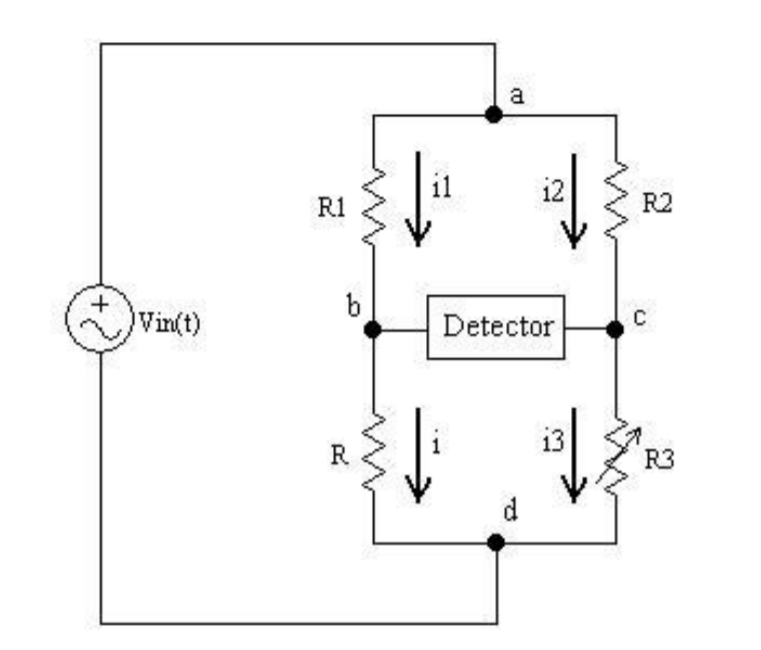
\includegraphics[width=0.6\textwidth]{6.png}
   \caption{Circuit diagram for Step 6}
\end{figure}  
For R1 and R2 1.2K\(\Omega\) resistors are used. For R3 6.8k\(\Omega\) resistor is used. Then 10k\(\Omega\) pot is properly adjusted so that the voltage between nodes b and c equals to 0. To learn the value of R3 the potentiometer is unplugged from the breadboard and its resistance is measured as "6.907k\(\Omega\)".

\section{Conclusion}
In conclusion, in experiment 3, "Introduction to Voltage, Current, and Resistance Measurements", as students, we have learned how to use different kinds of multimeters and potentiometers in general. The experiment was conducted in 7 steps. To determine the resistance of an unknown resistor, color code reading and multimeters measurement techniques are used. The resistance values of various potentiometers are obtained across different terminals and commented on. The internal batteries voltages of the analog and digital multimeters are measured, and it concluded that digital multimeters have higher measurement accuracy. The city line AC voltage is measured with analog multimeter. Voltage and current measurements are made on a circuit. The terminal characteristics of linear and non-linear resistors are observed. The properties of a potentiometer are explored on a resistive circuit. Current and voltage measurements are made for the diode on a circuit. The non-linear behavior of the diode component is observed in the data.  In this experiment, as students, we have experimented with how to use different kinds of multimeters for measurements and how to work with potentiometer components.
\section*{Appendix I}
Total time spent on/during:
\begin{itemize}
	\item Pre-lab preparation: 1 hours (including the preliminary work and simulations) 
	\item Experimental work: 2 hours (hours spent in lab)
	\item Report writing: 4.5 hours 
\end{itemize}
%++++++++++++++++++++++++++++++++++++++++
% References section will be created automatically 
% with inclusion of "thebibliography" environment
% as it shown below. See text starting with line
% \begin{thebibliography}{99}
% Note: with this approach it is YOUR responsibility to put them in order
% of appearance.

%\begin{thebibliography}{99}

%https://tr.overleaf.com/latex/templates/sample-lab-report-for-u-of-r-phys-349/pgsyqngcyjxk

%\end{thebibliography}


\end{document}


\begin{table}[H]
	\begin{center}
		\caption{Resistance reading by color code convention.}
		\vspace{2mm}
		\begin{tabular}{||c | c | c||} 
		 \hline
		 Color Order & Value & Tolerance \\ [0.5ex] 
		 \hline\hline
		 Brown / Black / Red / Gold & 1k\( \Omega \) & \( \% \) 5  \\ 
		 \hline
		 Yellow / Violet / Red / Gold & 4.7k\( \Omega \) & \( \% \) 5   \\
		 \hline
		 Brown / Grey / Orange / Gold & 18k\( \Omega \) & \( \% \) 5  \\ [1ex] 
		 \hline
		\end{tabular}
	\end{center}
	\end{table}

	\begin{figure}[H]
 		\centering
		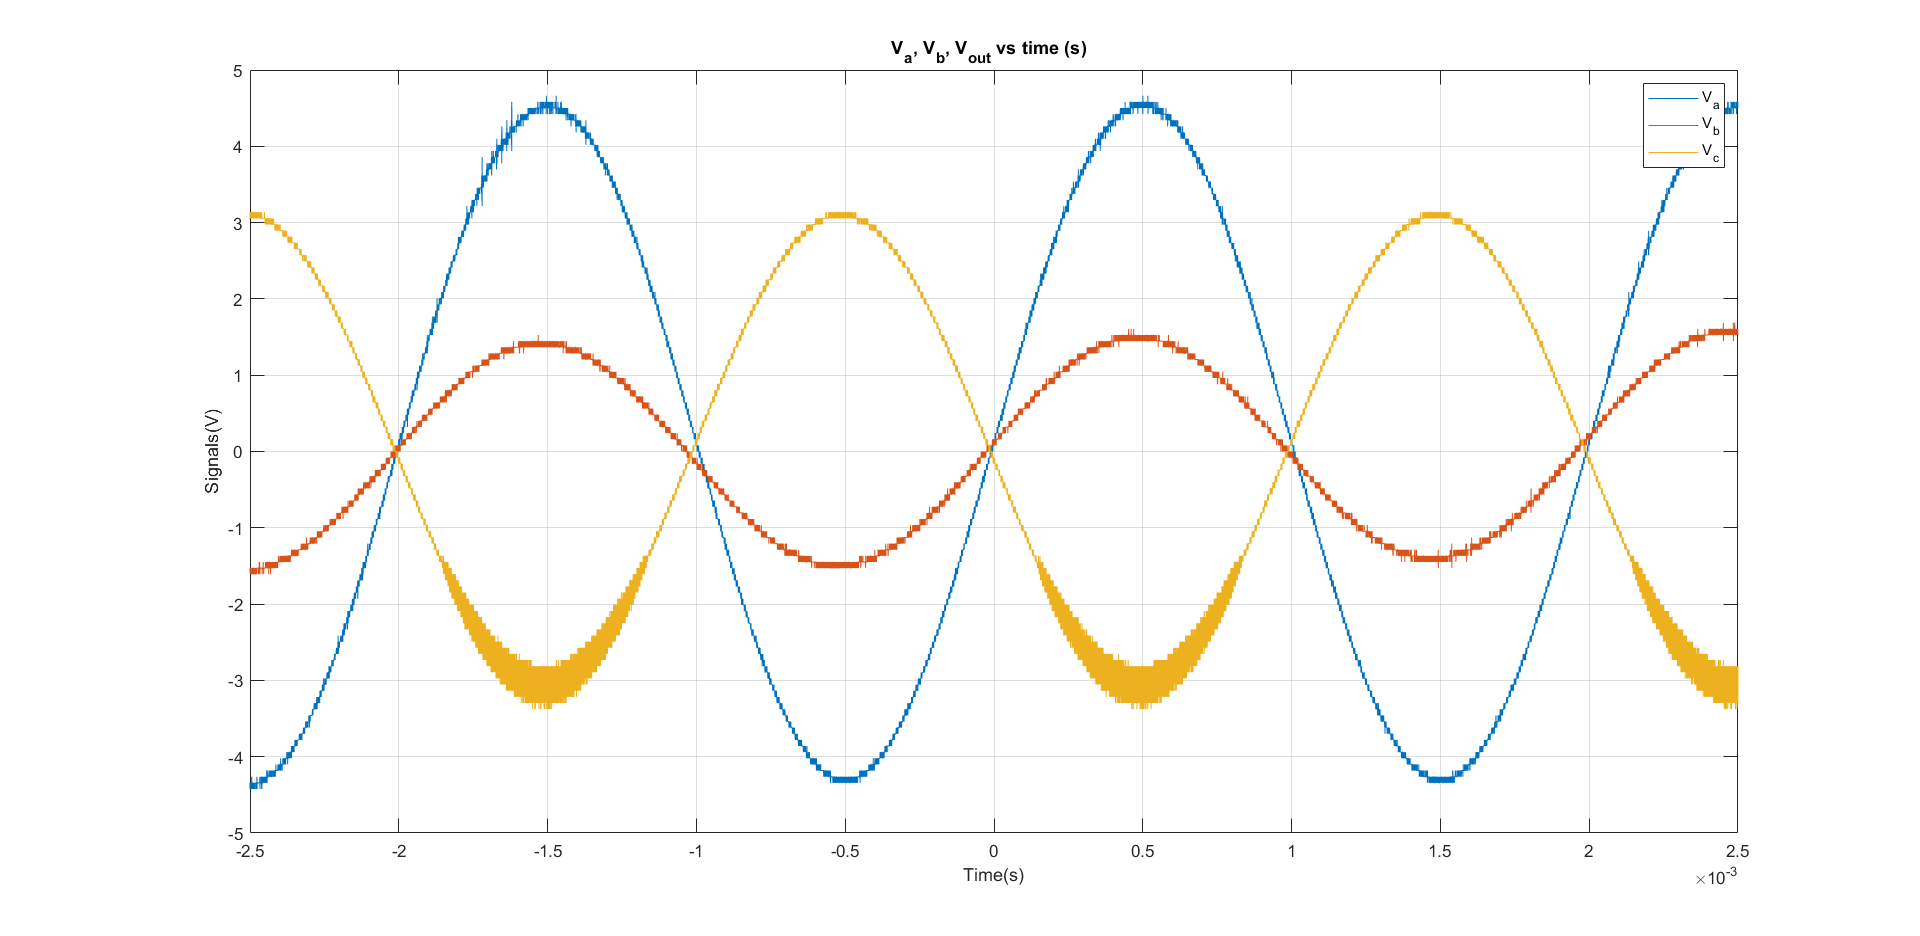
\includegraphics[width=0.6\textwidth]{5.png}
		\caption{Circuit schematic for the step 5}
	\end{figure} 

	\begin{figure}[htp] \centering{
		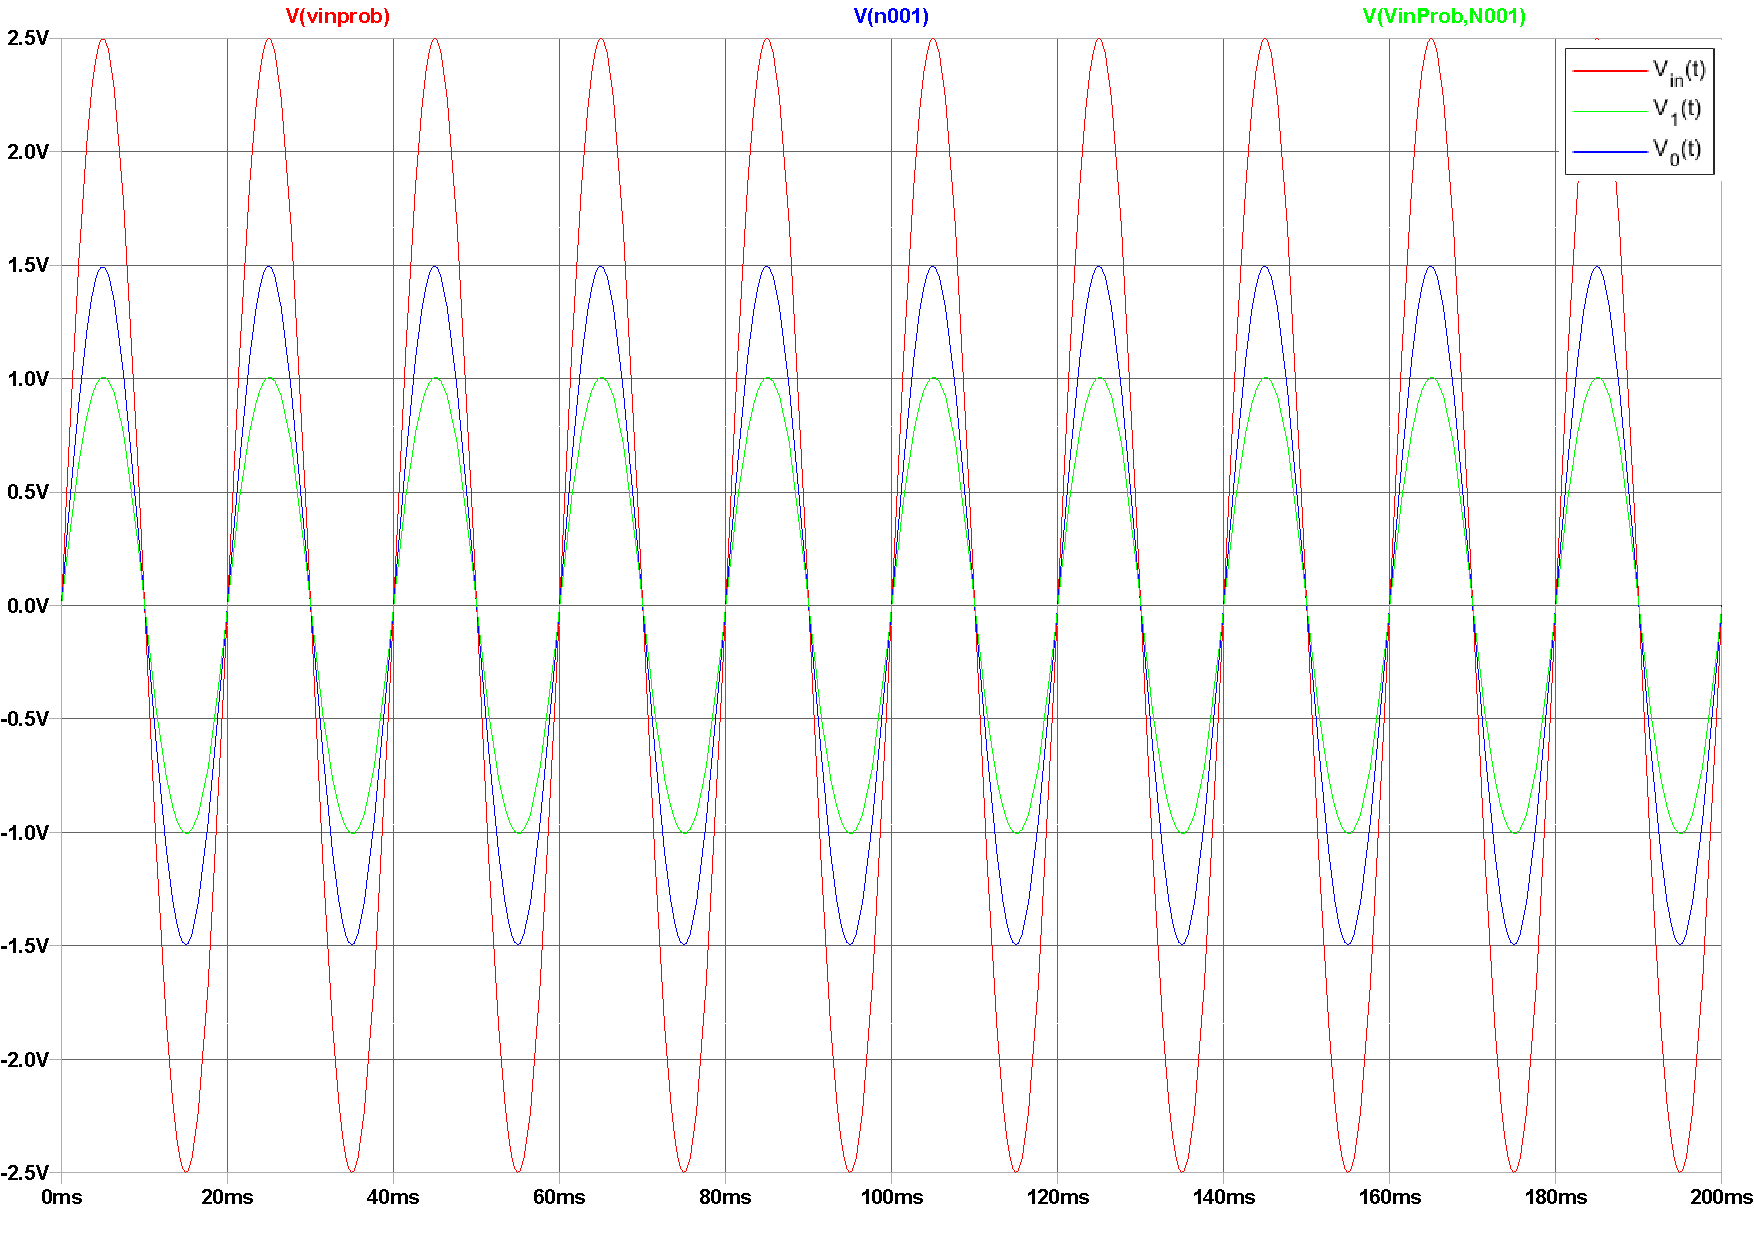
\includegraphics[scale=0.25]{2a_plot.pdf}}
		\caption{Experiment 2}
\end{figure}
	